\documentclass[PMO,authoryear,toc,lsstdraft]{lsstdoc}
\input{meta}

% Package imports go here.

% Local commands go here.

%If you want glossaries
%\input{aglossary.tex}
%\makeglossaries

\title{Rubin IPsec Tunnels}

% This can write metadata into the PDF.
% Update keywords and author information as necessary.
\hypersetup{
    pdftitle={Rubin IPsec Tunnels},
    pdfauthor={Julio Constanzo},
    pdfkeywords={}
}

% Optional subtitle
% \setDocSubtitle{A subtitle}

\author{%
Julio Constanzo
}

\setDocRef{ITTN-075}
\setDocUpstreamLocation{\url{https://github.com/lsst-it/ittn-075}}

\date{\today}

% Optional: name of the document's curator
% \setDocCurator{The Curator of this Document}

\setDocAbstract{%
The following document details the IPsec tunnel plan and deployment between the summit and SLAC
}

% Change history defined here.
% Order: oldest first.
% Fields: VERSION, DATE, DESCRIPTION, OWNER NAME.
% See LPM-51 for version number policy.
\setDocChangeRecord{%
  \addtohist{1}{2024-07-12}{First Release.}{Julio Constanzo}
}


\begin{document}

% Create the title page.
\maketitle
% Frequently for a technote we do not want a title page  uncomment this to remove the title page and changelog.
% use \mkshorttitle to remove the extra pages

% ADD CONTENT HERE
% You can also use the \input command to include several content files.

\section{Introduction}

This document details the overall deployment of the Rubin IPsec tunnels between the Rubin Pixel Zone network at Cerro Pachon in La Serena, Chile; and the protected enclave "Embargo" network at the SRCF (Stanford Research Computing Facility) inside the SLAC campus in California, US. 
It will also explain the physical connections and logical configurations made to accomplish the integration with the Rubin summit network, how access to the Long-Haul Network and how provides an encrypted channel between both sites. Bare in mind that all critical or confidential information that requires to be mentioned on this document will be only accesible through Vera C. Rubin Confluence page to protect the sensible data for security purposes.

If you require to access the detailed information please open a JIRA ticket or request access via the usual email or slack Rubin IT channels.
\section{Design}
The desing is the result of multiples discussions, were the goal was to provide a secure encrypted channel to transport the camera data from the top of the mountain to the enclave Embargo storage. Keep in mind that the data requires to flow from one site to another with a project time constrain of 7 seconds, making the task more interesting since now we need to encrypt the data before sending it to the other side of the tunnel, which takes a bit longer. 

In order to accomplish this challenge, and as mentioned before we choose the Arista DCS-7280CR3MK-32D4S with an encrypted module that could allow us to enable and setup IPSEC tunnels on top of the LHN. 
After Rubin purchased the equipment, two of them were sent to SLAC and the other two stayed at La Serena and then transported to the top of Cerro Pachón were the main telescope building and summit data center is located. These switches also work as our main TOR switches for the Rubin LFA cluster, same for SLAC and their Embargo storage cluster. This is made possible by using a mixture of MLAG + VVRP or VARP + OSPF.

\subsection{Hardware}
As was explained on \href{https://ittn-043.lsst.io/}{ittn-043}, the Rubin network is now using Arista Network as their core backbone equipment. As for the IPsec tunnels the hardware choosen was the Arista DCS-7280CR3MK-32D4S-R with an IPsec encryption module. 
To find the detailed datasheet please see the \href{https://www.arista.com/assets/data/pdf/Datasheets/7280R3-Data-Sheet.pdf}{Arista 7280R3 Data Sheet}.
The Arista 7280R3 Series with encryption delivers high performance, large packet buffers, high scale and availability with wire speed
AES-256-GCM encryption. 

\begin{itemize}
\item 32 x QSFP100, 4 x QSFP-DD
\item CPU Quad-Core x86
\item System Memory 64GB
\item Packet Buffer Memory 8GB
\item 1U
\item Wire speed L2 and L3 forwarding
\item Up to 4.8Tbps of wire speed performance with 8GB of buffer
\item Broad connectivity with 25G SFP, 100G QSFP and 400G OSFP / QSFP-DD
\item Encryption Support for TunnelSec (QSFP100 Ports)
\end{itemize}

\begin{figure}
    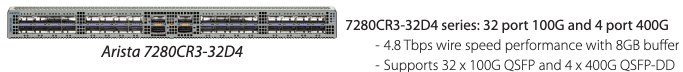
\includegraphics[width=16cm]{images/arista_datasheet01.png}
    \centering
    \caption{Arista DCS-7280CR3MK-32D4S}
  \end{figure}

There is a total of 4 Arista nodes, two of them are located in La Serena, Chile and the other two are at SLAC, US. 

\subsection{Licensing}

Arista has an easy way to manage their licenses and for the IPsec switches there are 3 main licenses that are running at this moment, been the IPsec license the most important one.

License feature: AHwSecSig
\begin{itemize}
\item License parameter:  *** info ommited *** 
\item Count: 1
\item Start: 2023-10-11 00:00:00
\item Expiration: 2123-09-17 00:00:00
\item Active: yes
\item License source: File
\end{itemize}

License feature: IPSec
\begin{itemize}
\item License parameter: None
\item Count: 4
\item Start: 2023-10-11 00:00:00
\item Expiration: 2123-09-17 00:00:00
\item Active: yes
\item License source: File
\end{itemize}

License feature: MACsec
\begin{itemize}
\item License parameter:  None
\item Count: 4
\item Start: 2023-10-11 00:00:00
\item Expiration: 2123-09-17 00:00:00
\item Active: yes
\item License source: File
\end{itemize}

The licenses were activated on all four switches, two of them in La Serena/Chile and the other two at SLAC/California and will not expire until 2123.

\subsection{Support}

Arista provides a TAC support team reachable via email, phone and online channels. We now have a good understanding on how to engage with them and scalate our issues. We have been working very closely to solve the many problems we encountered during the deployment of this project.
The Arista TAC team has proved to be an useful asset during the deployment of the IPsec tunnels environment.  

Note: The following definitions were extracted from the Arista official documentation from their latest release EOS64-4.32.1F that can be found \href{https://www.arista.com/en/um-eos/eos-data-plane-security#xx1009511}{here}

\newpage

\subsection{MLAG}
The Arista switches were configured in MLAG fashion to be used as TOR switches on both sites. Here a few benefits:

\begin{itemize}
    \item No wasted bandwidth with uplinks in Spanning Tree Blocking state
    \item Allows you to design non-blocking networks
    \item Maintains same level of resiliency with redundant paths available at all times
    \item No proprietary protocol used to connect an MLAG pair to servers or other switches. Interconnect to other switches or servers can use static LAG or IEEE 802.3ad LACP
    \item Spanning Tree Protocol can still be used in conjunction with MLAG to detect and handle any misconfigurations
\end{itemize}

\newpage

\subsubsection{Example of a MLAG configuration}
\begin{figure}
    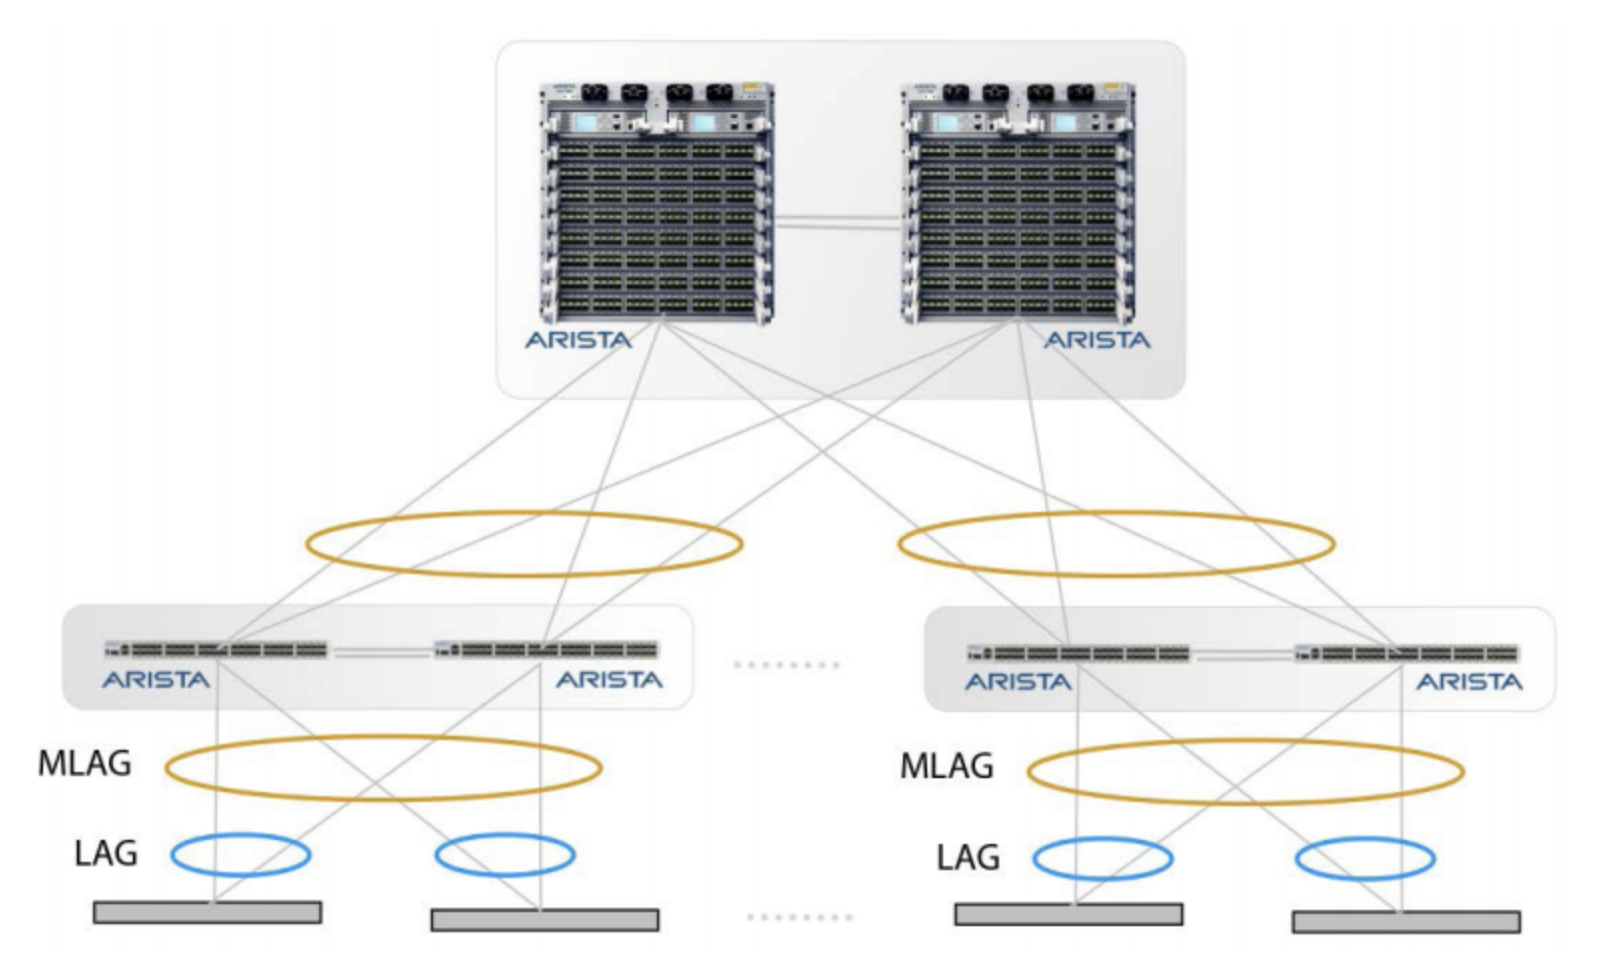
\includegraphics[width=16cm]{images/mlag.png}
    \centering
    \caption{Example of a MLAG configuration}
  \end{figure}

\subsection{IPSec}

The Arista DCS-7280CR3MK-32D4S provides IPSEC VTI mode which allows us to move the data using routing-based IPSEC, different from the conventional policy-based IPSEC.
The IPSec VTI tunnel mode support allows the customer to encrypt traffic transiting between two tunnel endpoints.

\begin{figure}
    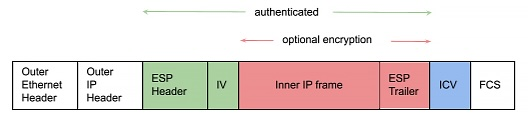
\includegraphics[width=16cm]{images/IPSEC_format.png}
    \centering
    \caption{IPSEC frame format}
  \end{figure}

\newpage

Internet Protocol Security (IPsec) is a protocol suite for securing Internet Protocol (IP) communications by authenticating and encrypting each IP packet of a communication session. IPsec includes protocols for establishing mutual authentication between agents periodically during the session and negotiation of cryptographic keys to be used during the session. IPsec supports network-level peer authentication, data origin authentication, data integrity, data confidentiality (encryption), and replay protection.
IPsec is used to protect data traffic between sites for example between Branch, HQ and Data center sites in an enterprise.
IPsec uses the following protocols to perform various functions:

\begin{itemize}
    \item Authentication Headers (AH): provides the connectionless integrity and data origin authentication for IP datagrams and provides protection against replay attacks.
    \item Encapsulating Security Payloads (ESP): provides the confidentiality, data-origin authentication, connectionless integrity and an anti-replay service (a form of partial sequence integrity).  
    Internet Key Exchange (IKE): is a key management protocol which provides security for virtual private networks' (VPNs) negotiations and network access to random hosts. It is also described as a method for exchanging keys for encryption and authentication over an unsecured medium, such as the Internet.
\end{itemize}
      
\subsection{Security Associations}
  
Security Associations (SA) provide the bundle of algorithms and data that provide the parameters necessary for AH and/or ESP operations. The Internet Security Association and Key Management Protocol (ISAKMP) provides a framework for authentication and key exchange, with actual authenticated keying material provided either by manual configuration with pre-shared keys, Internet Key Exchange (IKE and IKEv2) and other mechanisms. In order to decide what protection is to be provided for an outgoing packet, IPsec uses the Security Parameter Index (SPI), an index to the security association database (SADB), along with the destination address in a packet header, which together uniquely identify a security association for that packet. A similar procedure is performed for an incoming packet, where IPsec gathers decryption and verification keys from the security association database.
Full bidirectional communication requires at least two SAs, one for each direction. SA is defined by the following parameters:
  
\begin{itemize}
    \item Security Algorithms (AH) or Encapsulating Security Payloads (ESP) and keys.
    \item Mode: Tunnel or Transport.
    \item Key Management Method: Manual or IKE.
    \item Lifetime: Expressed in hours.
\end{itemize}
      
\subsection{Mode of Operation}
  
IPsec on Arista switches operates in tunnel mode. In tunnel mode, the entire IP packet is encrypted and/or authenticated. It is then encapsulated into a new IP packet with a new IP header.
  
Tunnel mode is used to create virtual private networks for network-to-network communications (for example, between routers to link sites). Tunnel mode is used for most network-to-network IPsec.

\subsection{Key Management}
  
Key management on Arista switches uses the Internet Key Exchange (IKE) method. Internet Key Exchange (IKE) supports automated generation and renegotiation of SAs (includes keys) between the devices at a configured interval so it is much more scalable and secure.  

IPsec needs SAs to define the algorithms and keys to use for protecting traffic. IKE establishes the SA so IPsec can protect traffic.
  
There are two IKE versions, IKEv1 and IKEv2. IKEv2 builds on IKEv1 but both are still widely used today.

\newpage

\subsubsection{IKEv1}
IKEv1 has two phases:
\begin{itemize}
    \item IKEv1 Phase 1
    \item IKEv1 Phase 2
\end{itemize}

\paragraph{IKEv1 Phase 1}
\begin{itemize}
    \item Uses main or aggressive mode exchange
    \item Negotiates IKE SA
    \item Used for control plane
    \item Peer authentication
\end{itemize}

\paragraph{IKEv1 Phase 2}
\begin{itemize}
    \item Uses quick mode exchange
    \item Negotiates IPsec SAs  
\end{itemize}
      
Note that there are two different SAs that are established. The IKE SA protects only the IKE key management session using the IKE policy defined. The policy should include the following parameters:
\begin{itemize}
    \item Encryption algorithm
    \item Hash MAC (HMAC) algorithm
    \item Peer authentication procedure
    \item Diffie-Hellman group for initial key exchange
    \item SA lifetime
\end{itemize}
          
IKE initially performs a Diffie-Hellman (DH) exchange at the start of the IKE session. A Diffie-Hellman (DH) exchange allows participants to produce a shared secret value. The strength of the technique is that it allows participants to create the secret value over an unsecured medium without passing the secret value through the wire. From that exchange, peers get shared keying material, which is then used for IKE encryption and integrity functions. The strength of that keying material can be used for faster performance, by choosing lower key sizes for Diffie-Hellman exchanges. The key length (strength) of Diffie-Hellman exchanges can be changed with the use of different DH groups.
  
When an IKE session's lifetime expires, a new Diffie-Hellman exchange is performed between peers and the IKE SA is re-established.
The IPsec protection policy resulting in IPsec SAs, defines the protection of network traffic. These IPsec SAs are usually negotiated over IKE sessions. The parameters that define the IPsec protection policy are:
\begin{itemize}
    \item Encryption Algorithm
    \item Hash MAC (HMAC) Algorithm  
\end{itemize}

Note that the key material for IPsec SA (also called Child SA) is derived from keying material from IKEv1 phase 1.

There are two different modes for phase 1:
\begin{itemize}
    \item Main Mode
    \item 6 packet exchange
    \item Full identity protection and better anti-DoS protection
    \item Aggressive Mode
    \item 3 packet faster session establishment
    \item Identities are exchanged in clear
    \item Weak DoS protection
\end{itemize}

\subsubsection{Authentication} 
\begin{itemize}
    \item Pre-Shared Keys (PSK): As the name suggests, a shared secret is distributed out-of-band to the peers. The peers use this information and nonce parameters to create a hash that is used to authenticate messages.
    \item PKI Certificates: Here, certificates of the peers are exchanged and hashes are calculated over these certificates to authenticate each other.
\end{itemize}

\subsubsection{IKEv2}
IKEv2 differs from IKEv1 in the following ways:
\begin{itemize}
    \item Faster setup because of reduced number of messages.
    \item More secure.
    \item ESP is reused for all IKEv2 messages.
    \item Suite-B support.
    \item There is no aggressive mode, so IKEv2 always provides identity protection.
    \item Additional authentication methods.
    \item Local and remote can use different authentication methods and use different pre-shared keys.
    \item Authentication is done unidirectionally in IKEv2. 
\end{itemize}
      
\subsection{Route-based VPN}
A route-based VPN employs routed tunnel interfaces as the endpoints of the virtual network. All traffic passing through a tunnel interface is placed into the VPN. Rather than relying on an explicit policy to dictate which traffic enters the VPN, static and/or dynamic IP routes are formed to direct the desired traffic through the VPN tunnel interface.
Since route-based VPNs support dynamic routing information through VPN tunnels. EOS supports only route based VPN for dynamic routing support and for easier configuration and management.
In route-based VPN, features like NAT, ACL, QoS is applied to packets before they are encrypted by applying these features to tunnel interface and can be applied to encrypted packets to applying these features on the physical interface carrying the tunnel traffic.
  
\subsubsection{Virtual Template Interface (VTI)}
A new tunnel interface type vti is introduced to represent the VPN tunnel. This tunnel interface will participate in the routing and any packets forwarded to it will be encrypted and forwarded to the other end of the tunnel. Note, that this does not add a new header to the packet.

\subsection{IPsec VTI Tunnels}

Since Rubin has a dedicated DWDM equipment between summit and base, with 4x 100Gbps free connections that were reserved for the Rubin IPsec switches point-to-point connections to the Rubin border routers for LHN access, we choose to create a total of four IPsec VTI tunnel. The decision was made due a configuration limitation, which explain that all IPsec tunnels required to be created under a physical interface but configured as a subinterface (This was learned via multiples troubleshooting sessions with Arista TAC)

These are the IDs of the Tunnels:
    \begin{enumerate}
        \item Tunnel101 - Primary link
        \item Tunnel102
        \item Tunnel103
        \item Tunnel104
    \end{enumerate}

The following high level diagram explain all the layers that exist between the Rubin IPsec switches and SLAC IPsec switches. 

\begin{figure}
    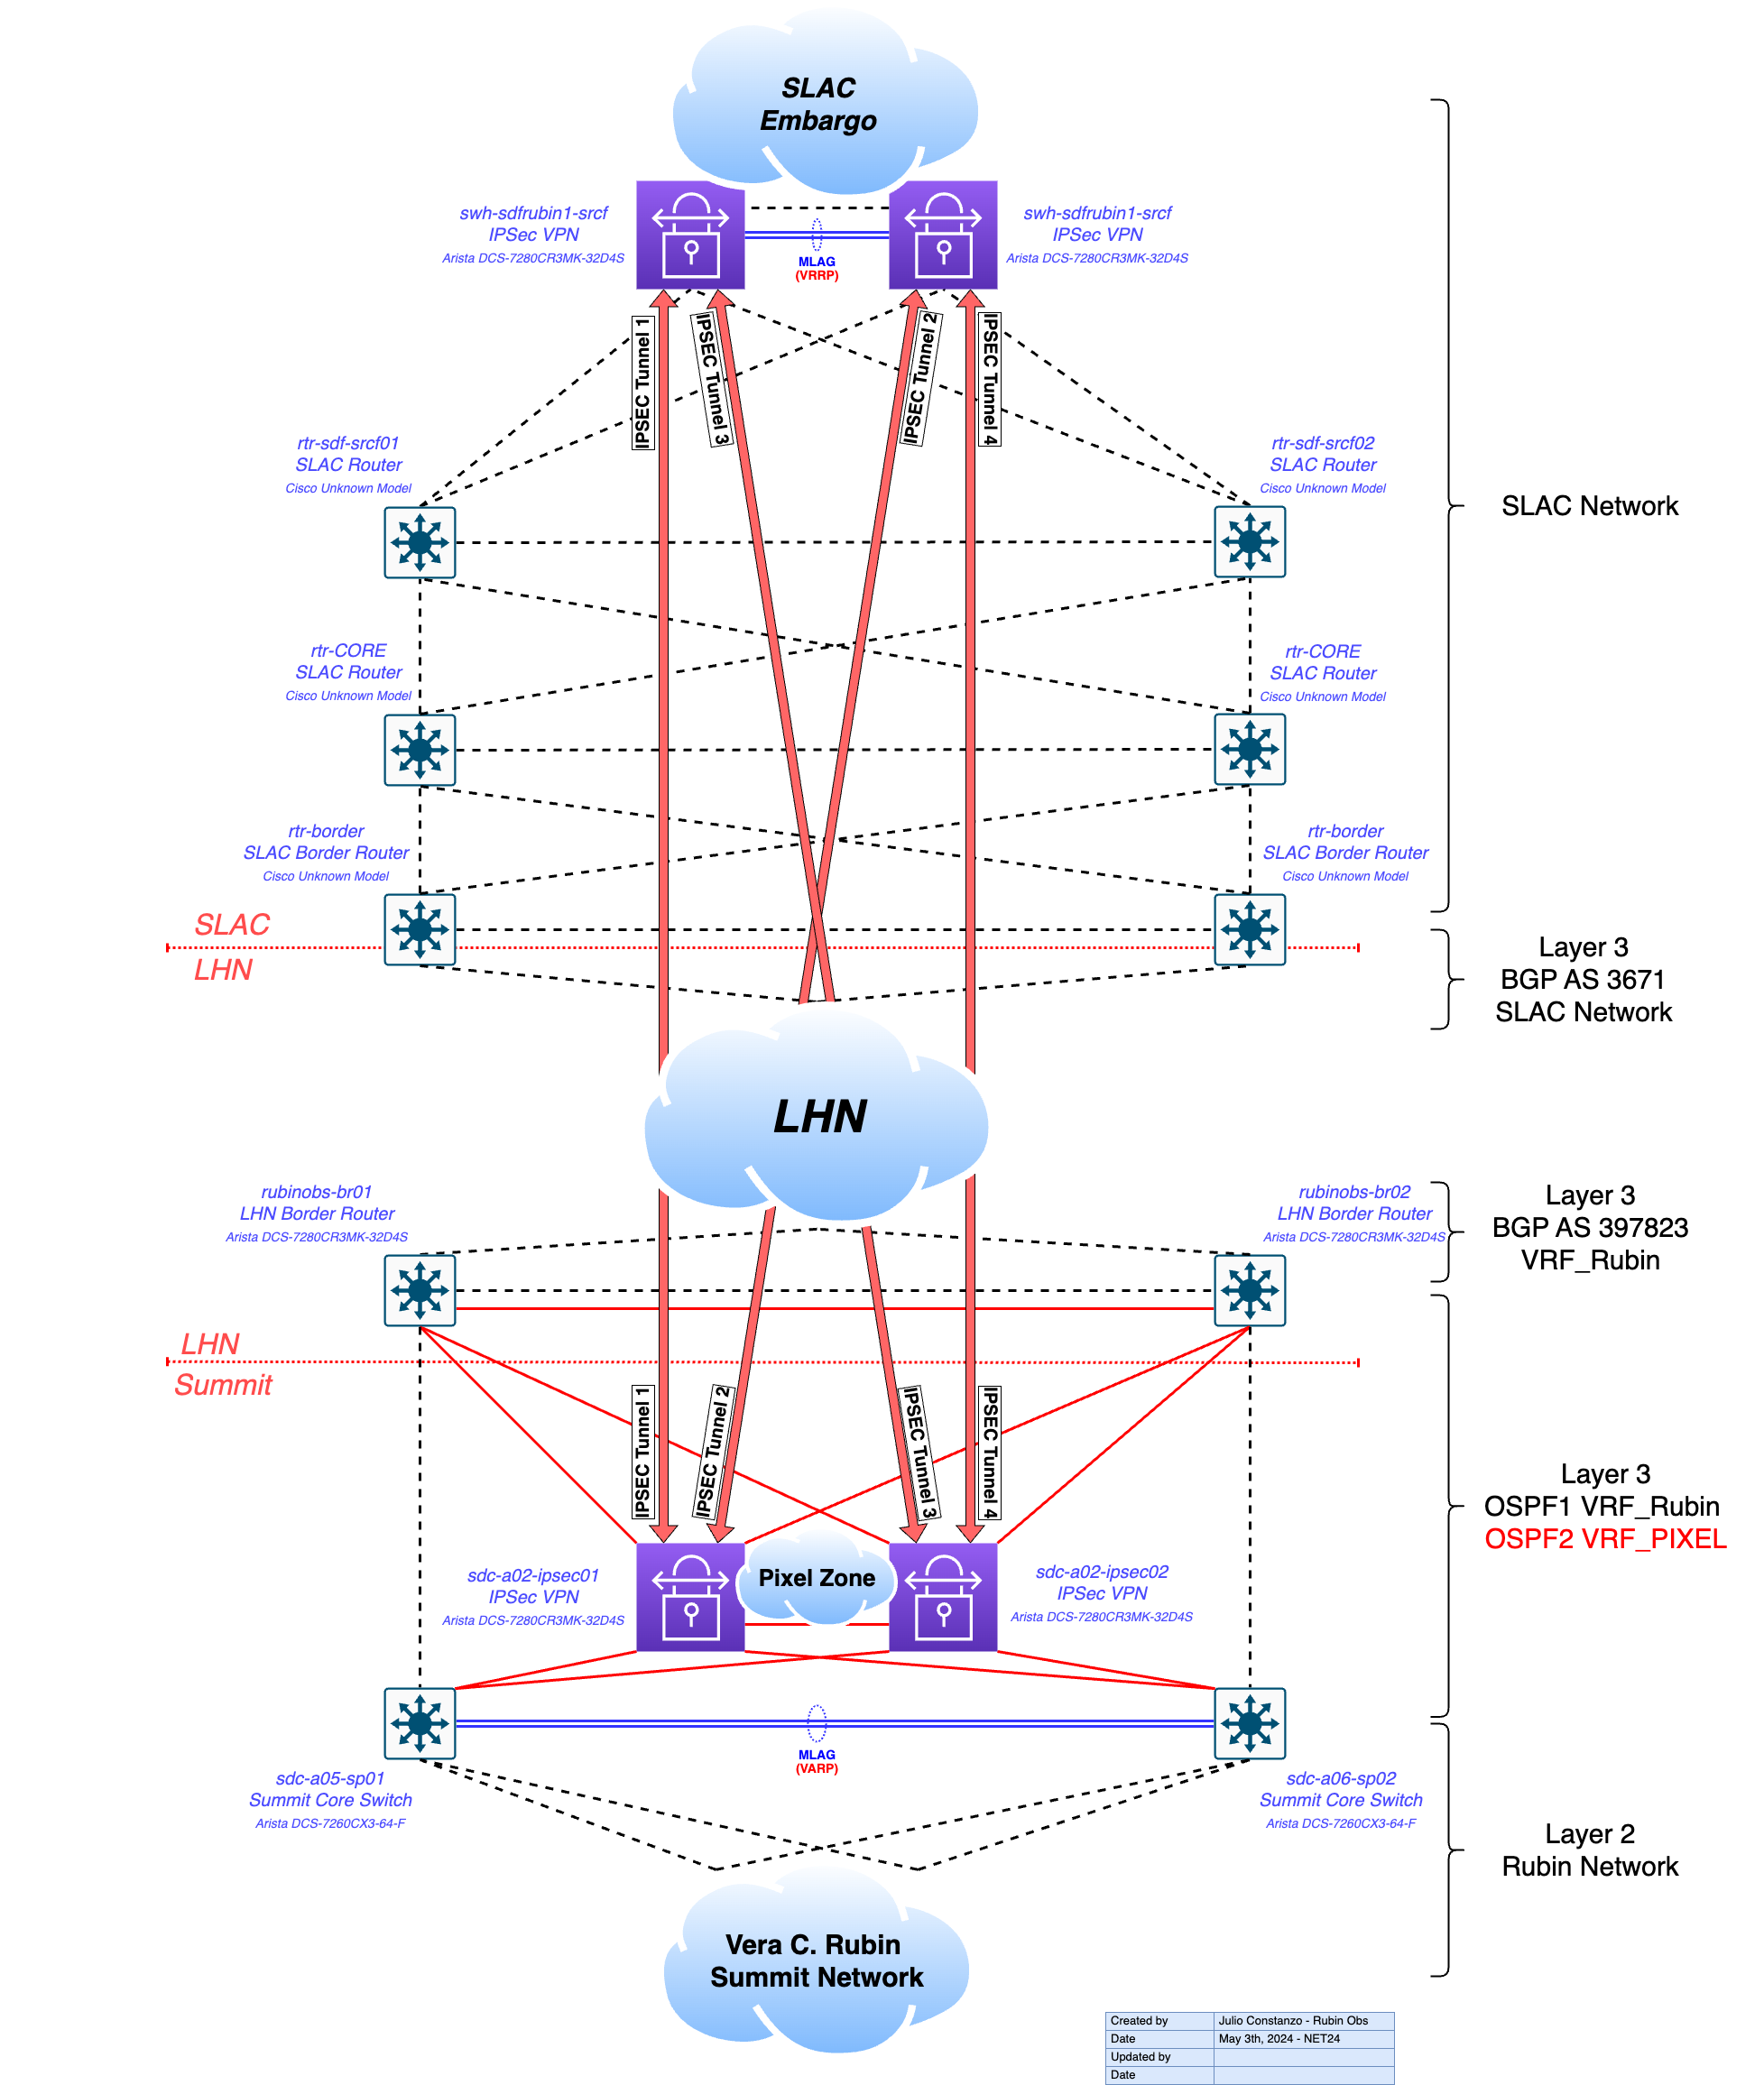
\includegraphics[width=16cm]{images/IPSec_Rubin_to_SLAC.png}
    \centering
    \caption{IPSEC Rubin to SLAC}
  \end{figure}

\section{IPsec Configuration}

As mentioned earlier on this document, the sensible configuration will not be disclosed on this document for security reasons, but it will be accesible via request and under Rubin Observatory security access policies.

The IPsec configuration is based on the following official Arista guide documentation release related to their latest EOS-4.32.1F software. The detailed documentation can be found \href{https://www.arista.com/en/um-eos/eos-data-plane-security#xx1007378}{here}

\subsection{Configuring IPsec}

This configuration will use the default IKE version 2 procedure. Keep in mind that this is an example configuration, and the actual configuration will not be disclosed on this document.

\begin{enumerate}
\item Use ip security command to enter IP security mode. 
    \begin{lstlisting}
        switch(config)# ip security
    \end{lstlisting}
\item To use IKE version 1, complete the following before completing the default IKE version the steps below.
        \begin{lstlisting}
        switch(config)# ip security
        switch(config-ipsec)# ike policy ike-peerRtr  
        switch(config-ipsec-ike)# version 1
        \end{lstlisting}
\item Create an IKE Policy to be used to communicate with the peer to establish IKE. You have the option of configuring multiple IKE policies.
    The default IKE Policy values are:
        \begin{itemize}
            \item Encryption: AES256 / AES128
            \item Integrity: SHA256 / SHA128
            \item DH group: Group 14
            \item IKE lifetime: 8 hours
        \end{itemize}
        \begin{lstlisting}
        switch(config-ipsec)# ike policy ike-router  
        switch(config-ipsec-ike)# encryption aes256  
        switch(config-ipsec-ike)# integrity sha256  
        switch(config-ipsec-ike)# dh-group 14  
        switch(config-ipsec-ike)# version 2
        \end{lstlisting}
\item If the router is behind a NAT, configure the local-id with the local public IP address. The public IP corresponds to the underlying interface over which the IKE communications are done with the peer.
        \begin{lstlisting}
        switch(config-ipsec-ike)# local-id <public ip address>
        \end{lstlisting}
\item Create an IPsec Security Association policy to be used in the data path for encryption and integrity. Use the option of enabling Perfect Forward Secrecy by configuring a DH group to the SA. In this example, AES256 is used for encryption, SHA 256 is used for integrity, and Perfect Forward Secrecy is enabled (the DH group is 14).
        \begin{lstlisting}
        switch(config-ipsec)# sa policy sa-vrouter  
        switch(config-ipsec-sa)# esp encryption aes256  
        switch(config-ipsec-sa)# esp integrity sha256  
        switch(config-ipsec-sa)# pfs dh-group 14  
        switch(config-ipsec-sa)# sa lifetime 2  
        switch(config-ipsec-sa)# exit
        \end{lstlisting}
\item Bind or associate the IKE and SA policies together using an IPsec profile. Provide a shared-key, which must be common on both peers. The default profile assigns default values for all parameters that are not explicitly configured in the other profiles. In this example, the IKE Policy ike-peerRtr and SA Policy sa-peerRtr are applied to profile peer-Rtr. Dead Peer Detection is enabled and configured to delete the connection when the peer is down for more than 50 seconds. The peer peer-Rtr is set to be the responder.
        \begin{lstlisting}
        switch(config-ipsec)# profile default
        switch(config-ipsec-profile)# ike-policy ikedefault
        switch(config-ipsec-profile)# sa-policy sadefault
        switch(config-ipsec-profile)# shared-key arista
        switch(config-ipsec-profile)# connection start
        switch(config-ipsec)# profile vrouter
        switch(config-ipsec-profile)# ike-policy ike-vrouter
        switch(config-ipsec-profile)# sa-policy sa-vrouter
        switch(config-ipsec-profile)# dpd 10 50 clear
        switch(config-ipsec-profile)# connection add
        \end{lstlisting}
\item Configure the WAN interface to be the underlying interface for the tunnel. You must specify an L3 address for the tunnel. If you do not, the switch cannot route packets using the tunnel.
        \begin{lstlisting}
        switch(config)# interface Et1  
        switch(config-if-Et1)# no switchport  
        switch(config-if-Et1)# ip address 1.0.0.1/24  
        switch(config-if-Et1)# mtu 1500     
        \end{lstlisting}
    Note: Rubin IPsec physical interfaces uses Jumbo frames with value 9214
\item Apply the IPsec profile to a new tunnel interface. You create the new tunnel interface as part of this step. You can configure the tunnel as a VTI IPsec tunnel. In this example, the new tunnel interface is Tunnel0. The new tunnel interface is configured to use IPsec. The other end of the tunnel also needs to be configured as a GRE-over-IPsec tunnel.
        \begin{lstlisting}
        switch(config)# interface tunnel0  
        switch(config-if-Tu0)# ip address 1.0.3.1/24  
        switch(config-if-Tu0)# mtu 1394  
        switch(config-if-Tu0)# tunnel source 1.0.0.1  
        switch(config-if-Tu0)# tunnel destination 1.0.0.2  
        switch(config-if-Tu0)# tunnel ipsec profile vrouter
        \end{lstlisting}
        Note: Rubin IPsec tunnel interfaces uses Jumbo frames with value 9214. Keep in mind that the IPsec add an overhead of 82 bytes.
\end{enumerate}    
    
\subsubsection{IPsec Example Configuration}
        \begin{lstlisting}
            ip security
            ike policy ikebranch1
            integrity sha256
            dh-group 15
            !
            sa policy sabranch1
            sa lifetime 2
            pfs dh-group 14
            !
            profile hq
            mode tunnel
            ike-policy ikebranch1
            sa-policy sabranch1
            connection add
            shared-key keyAristaHq
            dpd 10 50 clear
            !
            interface Tunnel1
            mtu 1404
            ip address 1.0.3.1/24
            tunnel source 1.0.0.1
            tunnel destination 1.0.0.2
            tunnel ipsec profile hq
            !
            interface Ethernet1
            no switchport
            ip address 1.0.0.1/24
            !        
        \end{lstlisting}

\subsection{Displaying IPsec Information}
    \begin{itemize}
        \item Use the command "show ip security connection  vrf all" to see all the secure connections status
        \item Use the "show ip security policy" command to display the IPsec policy information.
        \item Use the "show ip security profile" command to display the IPsec profile information.
        \item Use the "show kernel ipsec vrf all" command to displaya detailed view of the IPsec demon, state and parameters.
        \item Use the "show ip route vrf all" command to display the routing table list and check which IPsec tunnel is active.
    \end{itemize}
    
\section{IPsec Tunnels Deployment}

\subsection{Hardware Location}
At SLAC, the IPsec switches were installed at:
    \begin{itemize}
        \item SRCF located in row T1 and row T2
        \item Rack is commonly called "Embargo"
        \item Used as TOR switches for the Embargo storage cluster
    \end{itemize}

At Rubin, the IPsec switches were installed at:
    \begin{itemize}
        \item Summit Data Center at Cerro Pachón
        \item Rack SDC-A02
        \item Used as TOR switches for the Rubin LFA cluster
    \end{itemize}

\subsection{Rubin MLAG Configuration}
Both sites are using their respective nodes in MLAG fashion. To see the full MLAG configuration for Rubin IPsec MLAG setup, you can find it here: \href{https://confluence.lsstcorp.org/display/IT/ITTN-075+-+Rubin+IPsec+MLAG+Configuration}{Rubin IPsec MLAG Configuration}

\subsection{Rubin IPsec Configuration}

The IPsec configuration deployed for both sites can be found here: \href{https://confluence.lsstcorp.org/display/IT/ITTN-075+-+IPsec+Configuration}{Rubin IPsec Configuration}

\subsection{Rubin IPsec Tunnels and OSPF Configuration}
The IPsec configuration deployed for both sites can be found here: \href{https://confluence.lsstcorp.org/display/IT/ITTN-075+-+Rubin+IPsec+Tunnels+and+OSPF+Configuration}{Rubin IPsec Tunnels and OSPF Configuration}

\subsection{IPsec Tunnels Network Diagram}
The IPsec tunnels detailed diagram can be found here: \href{https://confluence.lsstcorp.org/display/IT/ITTN-075+-+Rubin+IPsec+Tunnels+Network+Diagram}{Rubin IPsec Tunnels Diagram}

\subsection{Summit to Base connection for IPsec switches}
The IPsec switches are directly connected to the base using the DWDM and into the Rubin border routers, the detailed diagram of those 4 x 100Gbps connections can be found here: \href{https://confluence.lsstcorp.org/display/IT/ITTN-075+-+Rubin+IPsec-to-BRs}{Rubin IPsec-to-BRs}
\section{Testing}

\subsection{Site to site reachability}
Once the tunnels were up, we start doing site to site ICMP tests to check if the both sites were reachable using the tunnels and jumbo frames. 

Note: As mentioned on the IPsec documentation, there's is a 82-bytes header to consider. 
82-bytes header + 8918-bytes  = 9K MTU 

    \begin{lstlisting}
sdc-a02-ipsec01#ping vrf VRF_PIXEL 10.77.77.0 source tunnel 101 df-bit size 8946
PING 10.77.77.0 (10.77.77.0) from 10.77.77.1 : 8918(8946) bytes of data.
8926 bytes from 10.77.77.0: icmp_seq=1 ttl=64 time=226 ms
8926 bytes from 10.77.77.0: icmp_seq=2 ttl=64 time=226 ms
8926 bytes from 10.77.77.0: icmp_seq=3 ttl=64 time=226 ms
8926 bytes from 10.77.77.0: icmp_seq=4 ttl=64 time=226 ms
8926 bytes from 10.77.77.0: icmp_seq=5 ttl=64 time=226 ms

--- 10.77.77.0 ping statistics ---
5 packets transmitted, 5 received, 0% packet loss, time 41ms
rtt min/avg/max/mdev = 226.414/226.433/226.486/0.026 ms, pipe 5, 
ipg/ewma 10.166/226.459 ms

sdc-a02-ipsec01#ping vrf VRF_PIXEL 10.77.77.2 source tunnel 102 df-bit size 8946
PING 10.77.77.2 (10.77.77.2) from 10.77.77.3 : 8918(8946) bytes of data.
8926 bytes from 10.77.77.2: icmp_seq=1 ttl=64 time=226 ms
8926 bytes from 10.77.77.2: icmp_seq=2 ttl=64 time=226 ms
8926 bytes from 10.77.77.2: icmp_seq=3 ttl=64 time=226 ms
8926 bytes from 10.77.77.2: icmp_seq=4 ttl=64 time=226 ms
8926 bytes from 10.77.77.2: icmp_seq=5 ttl=64 time=226 ms

sdc-a02-ipsec02#ping vrf VRF_PIXEL 10.77.77.4 source tunnel 103 df-bit size 8946
PING 10.77.77.4 (10.77.77.4) from 10.77.77.5 : 8918(8946) bytes of data.
8926 bytes from 10.77.77.4: icmp_seq=1 ttl=64 time=227 ms
8926 bytes from 10.77.77.4: icmp_seq=2 ttl=64 time=226 ms
8926 bytes from 10.77.77.4: icmp_seq=3 ttl=64 time=226 ms
8926 bytes from 10.77.77.4: icmp_seq=4 ttl=64 time=226 ms
8926 bytes from 10.77.77.4: icmp_seq=5 ttl=64 time=226 ms

--- 10.77.77.4 ping statistics ---
5 packets transmitted, 5 received, 0% packet loss, time 41ms
rtt min/avg/max/mdev = 226.401/226.468/226.560/0.055 ms, pipe 5, 
ipg/ewma 10.159/226.510 ms


sdc-a02-ipsec02#ping vrf VRF_PIXEL 10.77.77.6 source tunnel 104 df-bit size 8946
PING 10.77.77.6 (10.77.77.6) from 10.77.77.7 : 8918(8946) bytes of data.
8926 bytes from 10.77.77.6: icmp_seq=1 ttl=64 time=227 ms
8926 bytes from 10.77.77.6: icmp_seq=2 ttl=64 time=227 ms
8926 bytes from 10.77.77.6: icmp_seq=3 ttl=64 time=227 ms
8926 bytes from 10.77.77.6: icmp_seq=4 ttl=64 time=227 ms
8926 bytes from 10.77.77.6: icmp_seq=5 ttl=64 time=227 ms
\end{lstlisting}

\subsection{Routing Failover}

OSPF is configured to provide a routing failover when one of the physical interfaces or logical tunnels goes down.

The failover works as follows:

    \begin{enumerate}
        \item If Tunnel101 goes down, it will failover to Tunnel102, and continue to Tunnel103 if Tunnel102 goes down, until there's only Tunnel104 available.
        \item If one of the previous Tunnels goes back to normal, the routing table will be fill with the route of the Tunnel with the smaller ID value.
        \item Same behavior occurs if one of the physical links goes down.
    \end{enumerate}

This is how it looks when the primary link is up and run campaigns to encourage people to
    \begin{lstlisting}
    S   172.24.7.0/24 [1/0]
        via 10.77.77.0, Tunnel101, Static Interface IPsec tunnel index 101, 
        dst 134.79.22.230, src 139.229.140.1
    \end{lstlisting}

This is how it looks when the primary goes down and failover is engage.
    \begin{lstlisting}
    S   172.24.7.0/24 [1/0]
        via 10.77.77.2, Tunnel102, Static Interface IPsec tunnel index 102, 
        dst 134.79.22.226, src 139.229.140.3
    \end{lstlisting}

Note: 172.24.7.0/24 is the SLAC landing network.

\subsection{Performance}
The overall testing was made with two endpoint, one on each side behind the IPsec tunnels environment, each node connected using a 100Gbps NIC into the IPsec TOR switches.

Here's the Rubin endpoint TCP configuration for this node:

    \begin{lstlisting}
        [root@perfsonar1 sysctl.d]# cat 10-perfsonar.conf 
        # HEADER: This file was autogenerated at 2024-05-27 21:56:26 +0000
        # HEADER: by puppet.  While it can still be managed manually, it
        # HEADER: is definitely not recommended.
        net.core.rmem_max=268435456
        net.core.wmem_max=268435456
        net.ipv4.tcp_rmem=4096	87380	134217728
        net.ipv4.tcp_wmem=4096	65536	134217728
        net.ipv4.tcp_congestion_control=htcp
        net.core.default_qdisc=fq
        net.ipv4.conf.all.arp_announce=2
        net.ipv4.conf.all.arp_ignore=1
        net.ipv4.conf.all.arp_filter=1
        net.ipv4.conf.default.arp_filter=1
        net.ipv4.tcp_no_metrics_save=1
        \end{lstlisting}

The choosen tool for this test was iperf3. Here is the test results for 7 seconds and 60 seconds using above TCP configuration:

    \begin{lstlisting}
        [root@perfsonar1 sysctl.d]# iperf3 -c 172.24.7.31 -P 10 -t 7
        [SUM]  0.00-7.00  sec 12.8 GBytes 15.7 Gbits/sec  0      sender
        [SUM]  0.00-7.19  sec 12.8 GBytes 15.3 Gbits/sec         receiver
        iperf Done.

        [root@perfsonar1 sysctl.d]# iperf3 -c 172.24.7.31 -P 10 -t 60
        [SUM]  0.00-60.00 sec  138 GBytes 19.8 Gbits/sec 67384   sender
        [SUM]  0.00-60.19 sec  138 GBytes 19.7 Gbits/sec         receiver
        iperf Done.
    \end{lstlisting}

\newpage

Then we used another TCP congestion protocol: BBR 

    \begin{lstlisting}
        sysctl net.ipv4.tcp_congestion_control=bbr
    \end{lstlisting}

To learn more about BBR, please consider to check this document \href{https://internet2.edu/wp-content/uploads/2022/12/techex22-AdvancedNetworking-ExploringtheBBRv2CongestionControlAlgorithm-Tierney.pdf}{Exploring the BBRv2 Congestion Control
Algorithm for use on Data Transfer Nodes}

The Rubin and SLAC endpoints were set to use BBR as IPv4 TCP congestion protocol and this was the result for 7 seconds and 60 seconds:

    \begin{lstlisting}
    [root@perfsonar1 ~]# ./iperf3-static -c 172.24.7.31 -P 64 -t 7 -w 100M
    [SUM]  0.00-7.01  sec 36.1 GBytes 44.2 Gbits/sec 420779       sender
    [SUM]  0.00-7.24  sec 29.0 GBytes 34.4 Gbits/sec              receiver
    iperf Done.

    
    [root@perfsonar1 ~]# ./iperf3-static -c 172.24.7.31 -P 64 -t 60 -w 100M
    [SUM]  0.00-60.01 sec  342 GBytes 48.9 Gbits/sec 3028493       sender
    [SUM]  0.00-60.24 sec  332 GBytes 47.4 Gbits/sec         receiver
    iperf Done.
    \end{lstlisting}

    

\appendix
% Include all the relevant bib files.
% https://lsst-texmf.lsst.io/lsstdoc.html#bibliographies
\section{References} \label{sec:bib}
\renewcommand{\refname}{} % Suppress default Bibliography section
\bibliography{local,lsst,lsst-dm,refs_ads,refs,books}

% Make sure lsst-texmf/bin/generateAcronyms.py is in your path
\section{Acronyms} \label{sec:acronyms}
\addtocounter{table}{-1}
\begin{longtable}{p{0.145\textwidth}p{0.8\textwidth}}\hline
\textbf{Acronym} & \textbf{Description}  \\\hline

AES & Advanced Encryption Standard \\\hline
B & Byte (8 bit) \\\hline
CPU & Central Processing Unit \\\hline
DWDM & Dense Wave Division Multiplex \\\hline
EOS & Engineering Operations Services \\\hline
ESP & Early Science Program \\\hline
GRE & Generic Routing Encapsulation \\\hline
HQ & Head Quarters \\\hline
IP & Internet Protocol \\\hline
IPsec & Internet Protocol Security \\\hline
IT & Information Technology \\\hline
ITTN & IT Technote \\\hline
L2 & Lens 2 \\\hline
L3 & Lens 3 \\\hline
LAG & List of Acronyms and Glossary \\\hline
LFA & Large File Annex \\\hline
LHN & long haul network \\\hline
MAC & Media Access Control \\\hline
MLAG & Multi-chassis Link Aggregation \\\hline
MTU & Maximum Transmission Unit \\\hline
NAT & Network Address Translation \\\hline
OSPF & Open Short Path First \\\hline
PMO & Project Management Office \\\hline
QSFP & Quad Small Form Factor Plugable \\\hline
SA & System and Services Acquisition \\\hline
SLAC & SLAC National Accelerator Laboratory \\\hline
SPI & Schedule Performance Index \\\hline
SRCF & Stanford Research Computing Facility \\\hline
TAC & Time Allocation Committee \\\hline
TCP & Transmission Control Protocol \\\hline
US & United States \\\hline
VPN & virtual private network \\\hline
VRF & Virtual Routing and Forwarding \\\hline
WAN & Wide Area Network \\\hline
\end{longtable}

% If you want glossary uncomment below -- comment out the two lines above
%\printglossaries





\end{document}
